\documentclass[usenames, dvipsnames, aspectratio=32]{beamer}
\usepackage[utf8]{inputenc}
\usepackage[T1]{fontenc}
\usepackage[german]{babel}
\usepackage[defaultfam, regular]{montserrat}
\usepackage{csquotes}
\usepackage[normalem]{ulem}
\usepackage{latexsym,multicol,booktabs,miama}
\usepackage{setspace}
\usepackage{xcolor}
\usepackage{pgfplots,pgfpages}
\usepackage{tikz}
    \usetikzlibrary{calc}
\usepackage{amssymb,amsfonts,amsmath,amsthm,mathrsfs,mathptmx} 
\usepackage{graphicx,pstricks,listings,stackengine,multirow}
\usepackage{adjustbox}
\usepackage[backend=biber,bibencoding=utf8,urldateusetime=true,style=alphabetic,sorting=nyt,natbib=true]{biblatex}
\usepackage{../10_intermediate_defense/style}
\usepackage{hyperref}
    \hypersetup{colorlinks=true, citecolor=purple, filecolor=black, linkcolor=main, urlcolor=blue}

\setbeamertemplate{note page}[plain]
\setbeameroption{show notes on second screen=right}
\setbeamertemplate{note page}{\pagecolor{yellow!5}\vfill\insertnote\vfill}

\makeatletter
\def\beamer@setupnote{%
  \gdef\beamer@notesactions{%
    \beamer@outsideframenote{%
      \beamer@atbeginnote%
      \beamer@notes%
      \ifx\beamer@noteitems\@empty\else
      \begin{itemize}%
        \setlength{\itemsep}{.4em}% Abstand zwischen Items
        \setlength{\topsep}{.3em}% Abstand vor/nach der Liste
        \setlength{\parsep}{0pt}% Absatzabstand innerhalb eines Items
        \beamer@noteitems%
      \end{itemize}%
      \fi%
      \beamer@atendnote%
    }%
    \gdef\beamer@notesactions{}%
  }
}
\makeatother

\setbeamertemplate{bibliography item}{\insertbiblabel}
\setbeamertemplate{caption}[numbered]
\addbibresource{../../50_thesis/10_thesis/00_bibs/Extras.bib}
\addbibresource{../../50_thesis/10_thesis/00_bibs/Positive.bib}
\addbibresource{../../50_thesis/10_thesis/00_bibs/Eigenes.bib}


\author[Malte Grube]{\vspace*{-.8em}Malte Grube -- B.\,Sc. Informatik (2021)\inst{1}}
\title[]{LLMs in der Fragengenerierung}
\subtitle{--\;Endverteidigung\;--}
\institute[Universität Rostock]{
    \inst{1}
    \footnotesize{Betreuer: \textit{Prof.\,Dr. rer.nat. \uline{Clemens H. Cap}}} \vspace*{.25em} \\
    \textit{Jun.-Prof.in Dr.in \uline{Charlott Rubach}} \vspace*{-.25em}
}
\date{\today}

\def\cmd#1{\texttt{\color[RGB]{0, 0, 139}\footnotesize $\backslash$#1}}
\def\env#1{\texttt{\color[RGB]{0, 0, 139}\footnotesize #1}}

\lstdefinestyle{texstyle}{
    language=[LaTeX]TeX,
    basicstyle=\ttfamily\footnotesize,
    keywordstyle={\bfseries\color[RGB]{0, 0, 180}},
    keywordstyle=[2]{\slshape\color[RGB]{225, 140, 30}},
    morekeywords=[2]{,itemize, enumerate, equation, table, tabular},
    stringstyle=\color[RGB]{50, 50, 50},
    numbers=left,
    numberstyle=\footnotesize\color{gray},
    rulesepcolor=\color{red!20!green!20!blue!20},
    frame=shadowbox
}

\AtBeginBibliography{\scriptsize}

\begin{document}
{
\setbeamertemplate{headline}{}
\begin{frame}
    \vspace*{1em}
    \begin{figure}[htpb]
    \centering
    
\includegraphics[width=0.55\linewidth]{../10_intermediate_defense/logo.jpg}
    \end{figure}
    \vspace*{-1.5em}
    \titlepage
\end{frame}
}

\begin{frame}
    \tableofcontents[sectionstyle=show,subsectionstyle=show/shaded/hide,subsubsectionstyle=show/shaded/hide]
\end{frame}

\section{Einführung \& Problem}

\begin{frame}{Motivation \& Problemstellung I}
    \begin{itemize}
        \item \textbf{Motivation:} 
        \begin{itemize}
            \item Aktives Lernen $\to$ gezielte Fragen
            \item Anspruchsvolle Fragen $\to$ zeitaufwendig \cite{steuer_i_2021} 
        \end{itemize}
        \vspace{.5em}
        \item \textbf{Potenzial von LLMs:} Automatisierte Fragen- generierung $\to$ bessere Lehrmaterialien-Erstellung + Lernerfahrungen möglich \cite{naveed_comprehensive_2024}
    \end{itemize}
\end{frame}

\begin{frame}{Motivation \& Problemstellung II}
    \begin{itemize}
        \item \textbf{Problemstellung:} Qualität oft unklar $\to$ mangelnde systematische Evaluation über linguistische Tests hinaus \cite{horbach_linguistic_2020} 
            \note{\textbf{Problemstellung:}\\}
            \note[item]{P1: da auch die pädagogische Eignung bewertet werden muss über experten, was bis dato selten gemacht wurde \\}
        \begin{itemize}
            \item Selten pädagogische Bewertung \cite{zhuge_twinstar_2025,blobstein_angel_2023,scaria_how_2024}
                \note[item]{P1.1: manchmal nur linguistische Metriken genutzt, oder eben Expertenbewertung ohne Bloom \\}
            \item Mangelnde Performance bei höheren kognitiven Levels \cite{elkins_how_2023,scaria_how_2024}
                \note[item]{P1.2: die genutzten Modelle sind auch nicht die neuesten. \\}
            % angel gab es z.b.: gpt-3.5 basiert, super relatedness zu context (selbst bewertet), aber sehr niedrige kognitive levels (human eval)
            \item Relevanz $\neq$ Inhaltstreue \cite{elkins_how_2023,hang_mcqgen_2024,mi_comparative_2024}
                \note[item]{P1.3: korrektheit von Fragen elementar in Bildung; von interesse ist, wie man gut dies in form von inhaltstreue umsetzen kann; oft nur als future work erwähnt}
        \end{itemize}
        \vspace{.5em}
        \item \textbf{Forschungslücken:}
        \begin{itemize}
            \item Untersuchung der Inhaltstreue von LLMs
            \item Einhalten kognitiver Anforderungsniveaus
        \end{itemize}
    \end{itemize}
\end{frame}

\begin{frame}{Forschungsfragen}
    \begin{itemize}
        \item \textbf{RQ1:} Zu welchem Grad \textcolor{RedOrange!60}{halten sich LLMs} an den Inhalt verschiedener bereitgestellter \textcolor{RedOrange!60}{Lehrtexte} bei der Generierung von Fragen? \vspace{.5em}
        \item \textbf{RQ2:} Wie beeinflusst die \textcolor{RedOrange!60}{Beziehung} zwischen verschiedenen Frageformaten und den Levels der Bloom's Taxonomie die \textcolor{RedOrange!60}{pädagogische Wirksamkeit} von LLM-generierten Fragen?
    \end{itemize}
\end{frame}

\begin{frame}{Bloom's revised Taxonomy}
    \begin{itemize}
        \item \textbf{Pädagogische Relevanz:} Systematische Bewertung kognitiver Anforderungen von Fragen \cite{krathwohl_revision_2002}
    \end{itemize}
            \note[item]{Remembering: Abruf von Faktenwissen -- wiedergeben, nennen}
            \note[item]{Understanding: Bedeutung von Anweisungen erkennen -- erklären, beschreiben, zusammenfassen}
            \note[item]{Applying: Wissen in gegebenen Situationen anwenden -- anwenden, benutzen, durchführen}
            \note[item]{Analyzing: Material in Komponenten zerlegen -- untersuchen, vergleichen, kategorisieren}
            \note[item]{Evaluating: Urteile basierend auf Kriterien fällen -- bewerten, beurteilen, kritisieren}
            \note[item]{Creating: Elemente zu Ganzem zusammenfügen -- entwerfen, planen, entwickeln}
        \begin{figure}[htpb]
            \centering
            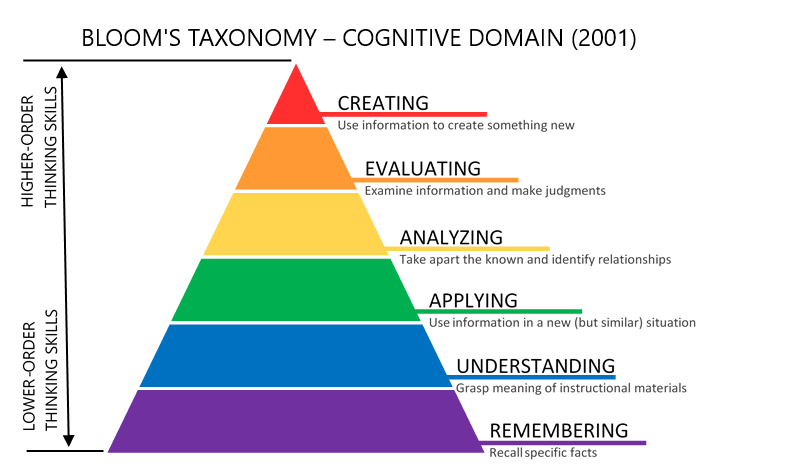
\includegraphics[width=0.6\linewidth]{../10_intermediate_defense/Blooms-Taxonomy.png}
            \caption{Kognitive Bloom-Hierarchie.}
            \label{fig:bloom}
        \end{figure}
\end{frame}

\begin{frame}{Herausforderungen der Literatur}
    \begin{itemize}
        \item \textbf{Veraltete Modelle} -- Kein Reasoning
            \note[item]{P1: pre-thinking basiert auf user prompt, damit modell verstehen kann, was der user will; wurde in der literatur noch nicht genutzt, sondern outdated models wie gpt-4/llama2}
        \item \textbf{Halluzinationen} -- Falsche Ausgaben
            \note[item]{P2: kann man minimieren durch kontext hinzugeben. durch pre-thinking kann das modell den kontext und die anforderungen hinterfragen}
        \item \textbf{Inhaltstreue} -- Forschung nötig
            \note[item]{P3: Inhaltstreue eher nebensache, mehr Bloom Fokus, linguistische metriken; mangel an systemen, welche die inhaltstreue von LLMs evaluieren}
        \item \textbf{Metriken im Fokus} -- Quantitative Evaluation
            \note[item]{P4: problematisch, da grundlegend linguistische \\ expertenbewertung notwendige evaluation bei aqg}
        \item \textbf{Expertenbewertung} -- Qualitative Evaluation
            \note[item]{P5: selten ausgiebig performt, weil es aufwendig ist}
        \item \textbf{Bloom's Taxonomy} -- Level Alignment \& \\ hohe kognitive Levels
            \note[item]{P6: schwerste levels, welche in related work mislungen; nicht immer bloom benutzt, und wenn, dann eher schlecht}
    \end{itemize}
\end{frame}

\begin{frame}{How to: Fleiss' Kappa}
    \begin{itemize}
        \item \textbf{Ziel:} Inter-Rater Reliability der Experten durch:
        \begin{align*}
            \kappa &= \frac{p_o - p_e}{1 - p_e}, \text{ mit}
        \end{align*}
        $p_o$ beobachtete Übereinstimmung, \\ $p_e$ erwartete Übereinstimmung durch Zufall, \\
        $N$ Anzahl der Fragen, \\
        $n$ Anzahl der Rater
            \note[item]{$n_{ij}$ Anzahl der Rater, die für Frage i das Rating j abgegeben haben}
            \note[item]{$k$ Menge der Auswahlmöglichkeiten 0,2,4,6,8,10}
            \note[item]{Nenner ist bei $p_o$ maximale Anzahl möglicher Übereinstimmungen von Raterpaaren über alle Fragen}
            \note[item]{$p_e$ wird jede Zählung quadriert, alle werden summiert (wie viele rater haben in kategorie $j$ zustimmung gegeben)}
        \begin{align*}
            p_o &= \frac{\sum_{i=1}^{N}\sum_{j=1}^{k} n_{ij}^2-N\cdot n}{N\cdot n\cdot (n-1)} \\
            p_e &= \sum_{j=1}^{k} p_j^2
        \end{align*}
    \end{itemize}
\end{frame}

\begin{frame}{Beispiel: Fleiss' Kappa}
    \begin{minipage}{.45\linewidth}
        \centering
        \begin{table}
            \begin{tabular}{cccc}
                \toprule
                \textbf{Q} & \textbf{R1} & \textbf{R2} & \textbf{R3} \\
                \midrule
                1 & Y & Y & Y \\
                2 & N & Y & N \\
                \bottomrule
            \end{tabular}
        \end{table}
        \vspace{-1em} 
        \begin{table}
            \begin{tabular}{cc}
                \toprule
                \textbf{Y} & \textbf{N} \\
                \midrule
                3 & 0 \\
                1 & 2 \\
                \midrule
                4 & 2 \\
                \bottomrule
            \end{tabular}
        \end{table}
        6 Ratings, somit: $\frac{4}{6}$ und $\frac{2}{6}$ \vspace{.5em} \\
        $\rightsquigarrow p_e=(\frac{4}{6})^2 + (\frac{2}{6})^2=\uline{0.55}$ 
    \end{minipage}%
    \begin{minipage}{.05\linewidth}
       \hfill 
    \end{minipage}
    \begin{minipage}{.48\linewidth}
        $N=2$ Fragen \& $n=3$ Rater \vspace{.5em} \\
        $\rightsquigarrow p_0=\frac{3^2+0^2+1^2+2^2-2\cdot 3}{2\cdot 3\cdot (3-1)}=\uline{0.66}$ \vspace{2em} \\
        Einsetzen in $\kappa$-Gleichung: \vspace{.5em} \\
        $\kappa=\frac{0.66 - 0.55}{1 - 0.55}=\uline{0.25}$
    \end{minipage}
\end{frame}

\section{Exp.\ 1 -- Inhaltstreue}

\begin{frame}{Experimentelles Design I}
    \begin{itemize}
        \item \textbf{Ziel:} Bewertung der Inhaltstreue LLM-\\ generierter Fragen
        \item \textbf{Materialien:} 3 Quellen -- ISO-OSI-Modell
        \begin{itemize}
            \item Script -- Prof. Cap's \enquote{Referenzarchitekturen} (DE)
            \item Transcript -- Audio-zu-Text (DE)  
            \item \enquote{Computer Networks} -- Textbook (EN)
        \end{itemize}
        \item \textbf{Exp 1a:} Originaltexte 
        \item \textbf{Exp 1b:} Manipuliertes Script 
    \end{itemize}
\end{frame}
\begin{frame}{Experimentelles Design II}
    \begin{itemize}
        \item 4 Large Language Models: 
            \begin{itemize}
                \item \textbf{DeepSeek:} R1 \textcolor{gray}{(Jan 2025)}
                \item \textbf{Anthropic:} Claude 3.7 Sonnet \textcolor{gray}{(Feb 2025)}
                \item \textbf{Google:} Gemini 2.5 Flash \textcolor{gray}{(Mar 2025)}
                \item \textbf{OpenAI:} o3 \textcolor{gray}{(Apr 2025)}
            \end{itemize}
        \item 2 Prompt-Strategien:
            \begin{itemize}
                \item \textbf{Einfach:} Weniger Anweisungen, keine Strukturierung, aber Formatvorlage + Material
                \note[item]{P2.1: generiere zum iso osi modell; korrekte antwort soll klar gekennzeichnet sein (wenn aus mehreren); kein abgrenzen von paragraphen durch strukturierung; klar und präzise Frage, kein weiterer Text soll generiert werden}
                \item \textbf{Komplex:} Rollenzuweisung, detaillierte Anweisungen, fordert nicht-triviales und kritisches Denken, Struktur durch Docstrings, Formatvorlage + Material 
                \note[item]{P2.2: rollenzuweisung (experte in generieren von kognitiv anspruchsvollen fragen, welche nicht triviales und analytisches denken fordern); untersuchen des osi texts; erfassen des wichtigen; nur fliesstext statt markdown}
                \note[item]{bei beiden prompts einheitliches outputformat, aber ohne festen fragetypen}
                \note[item]{präferenz von mcq in exp1}
            \end{itemize}
    \end{itemize}
\end{frame}

\begin{frame}{Datenerhebung \& Durchführung}
    \begin{itemize}
        \item \textbf{Python:} Automatisierte API-Ansteuerungen
        \item \textbf{Website-Prompting:} DeepSeek R1
        \item \textbf{Material:} Layer-weise Aufteilung
        \item \textbf{Resultierende \#Fragen:} 
    \end{itemize}
    \vspace{-.25em}
    \begin{align*}
        \textcolor{gray}{4 \text{ LLMs}\times 3 \text{ Inputs}\times 7 \text{ Layers}\times 2 \text{ Prompts}} &= \textcolor{gray}{168 \text{ Fragen}} \\
        \textcolor{gray}{4 \text{ LLMs}\times 1 \text{ Input}\times 7 \text{ Layers}\times 2 \text{ Prompts}} &= \textcolor{gray}{56 \text{ Fragen}}
    \end{align*}
\end{frame}

\begin{frame}[allowframebreaks]{Evaluations-Methodik}
    \begin{itemize}
        \item \textbf{Quantitativ:}
        \begin{itemize}
            \item \textbf{Semantic Similarity:} Generierte Frage vs. Originaltext
            \begin{itemize}
                \item[$\to$] Embedding-Modell \& Cosine Similarity \vspace{-.6em}
                % cosine sim
                % Bsp: (3,2) und (4,1) --> 3*4 + 2*1 / (sqrt(3^2+2^2) * sqrt(4^2+1^2)) = 14 / (sqrt(13) * sqrt(17)) = 0.94, sonst a mal b / ||a|| * ||b||
            \end{itemize}
            \begin{align*}
                \hspace{-3em}\cos(\vec{a}, \vec{b}) &= \frac{\vec{a} \cdot \vec{b}}{||\vec{a}|| \cdot ||\vec{b}||} 
            \end{align*}
            \item \textbf{Adherence Score:} o3 \& Claude 3.7 Sonnet Prompting
        \end{itemize}
        \item \textbf{Qualitativ:} Prof. Cap + 4 Experten des IuK 
        \begin{itemize}
            \item \textbf{Fleiss' Kappa:} Inter-Rater Reliability
            \item \textbf{Bewertungsrubrik:} 0-10 Punkte\,/\,Kategorie \& Frage:
            \item[] \textit{\textcolor{gray}{Relevance, Clarity, Answerability, Challenging, Value, Language \& Correctness vs. Manipulation Handling}}
        \end{itemize}
    \end{itemize}
\end{frame}

\begin{frame}{Quantitative Analyse -- Exp. 1a}
    \begin{figure}
        \centering
        \begin{tikzpicture}
            \node[inner sep=0pt, anchor=south west] (img) at (0,0)
                {\includegraphics[width=.85\linewidth]{../../40_evaluation/exp1/quantitative/plots/exp1a/combined_llm_vs_prompt_type.png}};
            \path[fill=white, fill opacity=0.55]
                (img.south west) --
                ($(img.south west)!0.5!(img.south east)$) --
                ($(img.north west)!0.5!(img.north east)$) --
                (img.north west) -- cycle;
        \end{tikzpicture}
        \vspace{-.5em}
        \caption{Heatmaps LLMs vs. Prompt-Typen (1a).}
        \label{fig:combined_llm_vs_prompt_type_a}
    \end{figure}
\end{frame}

\begin{frame}{Quantitative Analyse -- Exp. 1b}
    \begin{figure}
        \centering
        \begin{tikzpicture}
            \node[inner sep=0pt, anchor=south west] (img) at (0,0)
                {\includegraphics[width=.85\linewidth]{../../40_evaluation/exp1/quantitative/plots/exp1b/combined_llm_vs_prompt_type.png}};
            \path[fill=white, fill opacity=0.55]
                (img.south west) --
                ($(img.south west)!0.5!(img.south east)$) --
                ($(img.north west)!0.5!(img.north east)$) --
                (img.north west) -- cycle;
        \end{tikzpicture}
        \vspace{-.5em}
        \caption{Heatmaps LLMs vs. Prompt-Typen (1b).}
        \label{fig:combined_llm_vs_prompt_type_b}
    \end{figure}
\end{frame}

% \begin{frame}{Qualitative Analyse -- Exp. 1a}
%     \begin{itemize}
%         \item Supervisor-basiert: openai favorit bei correctness, transcript an sich favorit, script aber an sich auch genehm, jedoch ist google am schwächeln, vor allem im complex prompt
%         \item an sich mehr oder weniger knapp transcript am besten fuer alle kriterien ausser challenging, da ist script besser, daher auch bester mean total Score
%         \item common prompt am outperformen des complex prompts, ausser in challenging bei weitem
%     \end{itemize}
% \end{frame}

% \begin{frame}{Qualitative Analyse -- Exp. 1a}
%     \begin{itemize}
%         \item staff-basiert: favoritenrolle von openai nicht mehr so nuanciert, deepseek auch gute performance
%         \item hier script eher besser fuer viele kriterien ausser clarity knapp, answerability knapp, und language, da ist transcript besser, trotzdem aber besserer mean total score bei script ebenso
%         \item common prompt am outperformen des complex prompts, ausser in challenging bei weitem, genau wie bei supervisor
%     \end{itemize}
% \end{frame}

\newsavebox{\halfimgbox}
\newcommand{\includegraphicslefthalf}[2][]{%
  \sbox{\halfimgbox}{\includegraphics[#1]{#2}}%
  \clipbox{0pt 0pt {.5\wd\halfimgbox} 0pt}{\usebox{\halfimgbox}}%
}
\newcommand{\includegraphicsrighthalf}[2][]{%
  \sbox{\halfimgbox}{\includegraphics[#1]{#2}}%
  \clipbox{{.5\wd\halfimgbox} 0pt 0pt 0pt}{\usebox{\halfimgbox}}%
}

\begin{frame}{Qualitative Analyse -- Exp. 1a}
    \begin{figure}
        \centering
        \begin{minipage}[t]{0.49\linewidth}
            \centering
            \includegraphicslefthalf[width=1.6\linewidth]{../../40_evaluation/exp1/qualitative/plots/supervisor_exp1a_correctness_heatmaps.png}
        \end{minipage}\hfill
        \begin{minipage}[t]{0.49\linewidth}
            \centering
            \includegraphicslefthalf[width=1.6\linewidth]{../../40_evaluation/exp1/qualitative/plots/staff_exp1a_correctness_heatmaps.png}
        \end{minipage}
        \vspace{-.25em}
        \caption{Correctness Heatmaps -- Input Sources:\newline links Supervisor, rechts Staff.}
    \end{figure}
\end{frame}

\begin{frame}{Qualitative Analyse -- Exp. 1a}
    \begin{figure}
        \centering
        \hspace{-2em}
        \begin{minipage}[t]{0.49\linewidth}
            \centering
            \includegraphicsrighthalf[width=1.6\linewidth]{../../40_evaluation/exp1/qualitative/plots/supervisor_exp1a_correctness_heatmaps.png}
        \end{minipage}\hfill
        \begin{minipage}[t]{0.49\linewidth}
            \centering
            \includegraphicsrighthalf[width=1.6\linewidth]{../../40_evaluation/exp1/qualitative/plots/staff_exp1a_correctness_heatmaps.png}
        \end{minipage}
        \vspace{-.25em}
        \caption{Correctness Heatmaps -- Prompt Types:\newline links Supervisor, rechts Staff.}
    \end{figure}
\end{frame}

% \begin{frame}{Qualitative Analyse -- Exp. 1a}
%     \begin{itemize}
%         \item inter-rater agreement bei beiden gruppen und subexperimenten schlecht, da rubrik von staff members anders aufgegriffen wurde (zwischenwerte benutzt + rubrik nicht klar genug)
%     \end{itemize}
% \end{frame}

\begin{frame}{Qualitative Analyse -- Exp. 1a}
    \begin{table}
        \centering
        \caption{Inter-Rater Agreement Analyse (Exp1a). \newline Links: Staff. Rechts: Kombiniert.}
        \label{tab:iaa-exp1a-side-by-side}
        \begin{minipage}[t]{0.45\linewidth}
            \centering
            \scriptsize
            \begin{tabular}{lccc}
                \toprule
                \textbf{Kriterium} & \textbf{Fleiss' $\mathbf{\kappa}\uparrow$} & \textbf{Std} & \textbf{\#Raters} \\
                \midrule
                Relevance      & -0.085 & 1.92 & 4 \\
                Clarity        &  0.034 & 2.72 & 4 \\
                Answerability  &  0.015 & 2.84 & 4 \\
                Challenging    &  0.011 & 2.35 & 4 \\
                Value          & -0.010 & 3.23 & 4 \\
                Language       &  0.001 & 2.59 & 4 \\
                Correctness    & -0.052 & 2.67 & 4 \\
                \bottomrule
            \end{tabular}
        \end{minipage}\hfill
        \begin{minipage}[t]{0.45\linewidth}
            \centering
            \scriptsize
            \begin{tabular}{ccc}
                \toprule
                \textbf{Fleiss' $\mathbf{\kappa}\uparrow$} & \textbf{Std} & \textbf{\#Raters} \\
                \midrule
                -0.046 & 1.88 & 5 \\
                 0.077 & 2.68 & 5 \\
                 0.054 & 2.77 & 5 \\
                 0.014 & 2.61 & 5 \\
                 0.012 & 3.34 & 5 \\
                 0.043 & 2.53 & 5 \\
                -0.022 & 2.56 & 5 \\
                \bottomrule
            \end{tabular}
        \end{minipage}
    \end{table}
\end{frame}

\begin{frame}{Qualitative Analyse -- Exp. 1b}
\begin{table}[htbp]
    \centering
    \caption{Manipulation Handling Analyse via LLM \& Prompt Type. Links: Supervisor. Rechts: Staff.}
    \label{tab:exp1b-manipulation-handling-side-by-side}
    \begin{minipage}[t]{0.66475\linewidth}
        \centering
        \scriptsize
        \resizebox{\linewidth}{!}{%
        \begin{tabular}{llccc}
            \toprule
            & & \multicolumn{3}{c}{\textbf{Supervisor Scores}} \\
            \cmidrule(lr){3-5}
            \textbf{LLM} & \textbf{Prompt Type} & \textbf{Mean} & \textbf{Std} & \textbf{Median} \\
            \midrule
            \multirow{2}{*}{Anthropic} 
            & Common & 0.0 & 0.0 & 0.0 \\
            & Complex & \textbf{2.5} & 3.54 & \textit{2.5} \\
            \midrule
            \multirow{2}{*}{DeepSeek} 
            & Common & 2.5 & 3.54 & 2.5 \\
            & Complex & 2.5 & 3.54 & 2.5 \\
            \midrule
            \multirow{2}{*}{Google} 
            & Common & 0.0 & 0.0 & 0.0 \\
            & Complex & \textbf{2.5} & 3.54 & \textit{2.5} \\
            \midrule
            \multirow{2}{*}{OpenAI} 
            & Common & 0.0 & 0.0 & 0.0 \\
            & Complex & 0.0 & --- & 0.0 \\
            \bottomrule
        \end{tabular}}
    \end{minipage}\hfill
    \begin{minipage}[t]{0.31625\linewidth}
        \centering
        \scriptsize
        \resizebox{\linewidth}{!}{%
        \begin{tabular}{ccc}
            \toprule
            \multicolumn{3}{c}{\textbf{Staff Scores}} \\
            \cmidrule(lr){1-3}
            \textbf{Mean} & \textbf{Std} & \textbf{Median} \\
            \midrule
            % Anthropic
            2.50 & 4.63 & 0.0 \\
            \textbf{7.25} & 2.55 & \textit{8.0} \\
            \midrule
            % DeepSeek
            3.38 & 4.37 & 1.5 \\
            \textbf{5.12} & 4.64 & \textit{5.5} \\
            \midrule
            % Google
            3.50 & 4.66 & 0.5 \\
            \textbf{7.88} & 3.00 & \textit{8.5} \\
            \midrule
            % OpenAI
            2.50 & 4.63 & 0.0 \\
            \textbf{5.00} & 3.93 & \textit{4.0} \\
            \bottomrule
        \end{tabular}}
    \end{minipage}
\end{table}
\end{frame}

\begin{frame}{Qualitative Analyse -- Exp. 1b}
\begin{table}[H]
   \centering
   \caption{Inter-Rater Agreement Analyse (Exp1b).}
   \label{tab:iaa-staff-1b}
   \resizebox{.9\linewidth}{!}{%
   \begin{tabular}{lcccc}
        \toprule
        \textbf{Manipulation Handling} & \textbf{Fleiss' $\mathbf{\kappa}\uparrow$} & \textbf{Std} & \textbf{\#Items} & \textbf{\#Raters} \\
        \midrule
        Nur Staff & 0.014 & 4.31 & 16 & 4 \\
        Mit Supervisor kombiniert & 0.036 & 4.21 & 15 & 5 \\
        \bottomrule
   \end{tabular}}
\end{table}
\end{frame}

\section{Exp.\ 2 -- Bloom-Analyse}

\begin{frame}[allowframebreaks]{Experimentelles Design}
    \begin{itemize}
        \item \textbf{Ziel:} Auswertung Bloom-Level\,/\,Alignment
        \item \textbf{Materialien:} Alle ISO-OSI Script Layer
        \item \textbf{Fragetypen:} Multiple-Choice \& Freitextfragen
        \item \textbf{Prompting:} Rollenzuweisung, klare Formatvorgaben, Angabe von Fragetyp, Bloom-Level, oder beidem:
    \end{itemize}
    \begin{align*}
        \textcolor{gray}{4 \text{ LLMs}\times 2 \text{ Fragetypen}\times 6 \text{ Runs}} &= \textcolor{gray}{48 \text{ Fragen}} \\
        \textcolor{gray}{4 \text{ LLMs}\times 6 \text{ Bloom-Levels}} &= \textcolor{gray}{24 \text{ Fragen}} \\
        \textcolor{gray}{4 \text{ LLMs}\times 2 \text{ Fragetypen}\times 6 \text{ Bloom-Levels}} &= \textcolor{gray}{48 \text{ Fragen}}
    \end{align*}
\end{frame}

\begin{frame}{Evaluations-Methodik}
    \begin{itemize}
        \item \textbf{Qualitativ:} Ausschließlich Nutzen der Rubrik mit \textit{Bloom's Level} statt \textit{Correctness}
        \item \textbf{Umsetzung:} 3 Studenten von Prof. Rubach \& Inter-Rater Agreement (Fleiss' Kappa)
    \end{itemize}
\end{frame}

\begin{frame}{Qualitative Analyse -- Exp. 2}
\begin{table}[htbp]
    \centering
    \caption{Bloom Scores via LLM und Sub-Experiment.}
    \label{tab:exp2-llm-experiment-bloomslevel}
    \resizebox{\textwidth}{!}{%
    \begin{tabular}{lccccccccc}
        \toprule
        \multirow{2}{*}{\textbf{LLM}} & \multicolumn{3}{c}{\textbf{Mean}} & \multicolumn{3}{c}{\textbf{Std}} & \multicolumn{3}{c}{\textbf{Median}} \\
        \cmidrule(lr){2-4} \cmidrule(lr){5-7} \cmidrule(lr){8-10}
        & \textbf{Exp2a} & \textbf{Exp2b} & \textbf{Exp2c} & \textbf{Exp2a} & \textbf{Exp2b} & \textbf{Exp2c} & \textbf{Exp2a} & \textbf{Exp2b} & \textbf{Exp2c} \\
        \midrule
        Anthropic & \textbf{4.96} & 8.33 & 8.75 & 2.57 & 4.08 & 2.26 & \textit{7.0} & 10.0 & 10.0 \\
        DeepSeek  & 2.83 & 8.33 & 8.75 & 1.50 & 4.08 & 2.26 & 3.0 & 10.0 & 10.0 \\
        Google    & 4.54 & 8.33 & \textbf{9.58} & 2.53 & 4.08 & 1.44 & 3.0 & 10.0 & 10.0 \\
        OpenAI    & 3.67 & \textbf{10.00} & 7.50 & 2.78 & 0.00 & 3.99 & 3.0 & 10.0 & 10.0 \\
        \bottomrule
    \end{tabular}}
\end{table}
% ohne geg. bloom level: 1 --> 1.5p
% 2 --> 3p; 3 --> 4.5p; 4 -> 7p
% 5 --> 8.5p; 6 --> 10p

% mit bloom: getroffen --> 10p;
% eins vorbei: 5p; sonst: 0
\end{frame}

\begin{frame}{Qualitative Analyse -- Exp. 2}
\begin{table}[htbp]
    \centering
    \caption{Vergleich von Bloom Scores zwischen Fragetyp \& Sub-Experiment (2a und 2c).}
    \label{tab:exp2-questiontype-experiment-bloomslevel}
    \resizebox{.9\textwidth}{!}{%
    \begin{tabular}{lcccccc}
        \toprule
        \multirow{2}{*}{\textbf{Fragetyp}} & \multicolumn{2}{c}{\textbf{Mean}} & \multicolumn{2}{c}{\textbf{Std}} & \multicolumn{2}{c}{\textbf{Median}} \\
        \cmidrule(lr){2-3} \cmidrule(lr){4-5} \cmidrule(lr){6-7}
        & \textbf{Exp2a} & \textbf{Exp2c} & \textbf{Exp2a} & \textbf{Exp2c} & \textbf{Exp2a} & \textbf{Exp2c} \\
        \midrule
        Multiple-Choice & 2.42 & 7.92 & 1.23 & 3.27 & 2.25 & 10.0 \\
        Open-Ended      & \textbf{5.58} & \textbf{9.38} & 2.38 & 1.69 & \textit{7.00} & 10.0 \\
        \bottomrule
    \end{tabular}}
\end{table}
\end{frame}

\begin{frame}{Qualitative Analyse -- Exp. 2}
\begin{table}[H]
    \centering
    \caption{Inter-Rater Agreement Analyse (Exp2).}
    \label{tab:iaa-students-exp2}
    \resizebox{.8\textwidth}{!}{%
    \begin{tabular}{lcccc}
        \toprule
        \textbf{Kriterium} & \textbf{Fleiss' $\mathbf{\kappa}\uparrow$} & \textbf{Std} & \textbf{\#Items} & \textbf{\#Raters} \\
        \midrule
        Relevance          & 0.056 & 1.71 & 40 & 3 \\
        Clarity            & -0.058 & 1.61 & 40 & 3 \\
        Answerability      & 0.179 & 1.90 & 39 & 3 \\
        Challenging        & 0.270 & 2.52 & 40 & 3 \\
        Value              & -0.256 & 1.72 & 40 & 3 \\
        Language           & 0.016 & 1.95 & 40 & 3 \\
        Bloom Rating       & 0.397 & 1.67 & 40 & 3 \\
        \bottomrule
    \end{tabular}}
\end{table}
\end{frame}

\section{Schlusswort}

\begin{frame}{Hauptergebnisse zu RQ1 I}
    \begin{itemize}
        \item \textbf{LLMs erstellen inhaltsgetreue Fragen} unter bestimmten Bedingungen
            \note[item]{P1: adherence score zeigte recht deutlich, dass die Fragen inhaltlich gut waren}
            \note[item]{sentence transformer aber ungeeignet für lange Texte und strukturiertes}
        \item \textbf{Common Prompt > Complex} meistens
            \note[item]{P2: sowohl bei quantitativ als auch qualitativ; bei qualitativ nur complex besser in challenging mit einbußen}
            \note[item]{überladener/weniger präziser prompt folgert nicht unbedingt besseres}
        \item Script vs. Transcript oft eng beieinander, wobei \\
        \textbf{Staff:} Script vs. \textbf{Supervisor:} Transcript
            \note[item]{P3: transcript bei cap bestes in clarity,answerability und correctness, niedrigstes in challenging (bei beiden)}
            \note[item]{script bei staff ausgeglichen mit höchstem total score, script bei staff das effektivere material}
        \item OpenAI \& DeepSeek \textbf{konsistenter}
            \note[item]{anthropic \& google variabler... teils sprachlich komplex oder mit fehlerhaften/erfundenen optionen}
    \end{itemize}
\end{frame}

\begin{frame}{Hauptergebnisse zu RQ1 II}
    \begin{itemize}
        \item \enquote{Basierend auf dem gegebenen Text} \\ $\Rightarrow$ oft bei Deepseek \& Google
        \item \textbf{Teilweise Erkennung} von Manipulationen: \newline OpenAI \& DeepSeek niedrige \textit{Adherence Scores} beim komplexen Prompt
            \note[item]{P2: Anthropic \& Google folgen hierbei häufiger}
        \item \textbf{Kleine Stichprobe} (16/56) und \textbf{geringe IRR} \\
            \note[item]{P3: deswegen google und anthropic hier besser}
        $\Rightarrow$ Inkonsistente Trends quantitativ \& qualitativ
        \item \textbf{Bloom's Taxonomy} essentiell für gute + anforderungs-gesteuerte Fragen
    \end{itemize}
        \note[item]{also klappt dann gut, wenn man klare anweisungen gibt + strukturiertes material}
        \note[item]{DeepSeek und OpenAI dabei am robustesten gewesen grundlegend}
        \note[item]{IAA war sehr niedrig, die rubrik und pflichten der bewerter muessen refined werden}
        \note[item]{da fragen nicht so challenging (auch nicht so recht bei complex prompt), ist die wichtigkeit von blooms taxonomy vertreten}
\end{frame}

\begin{frame}{Hauptergebnisse zu RQ2 I}
    \begin{itemize}
        \item Bloom-Level-Spezifikation $\Rightarrow$ \textbf{hohe Adhärenz}
        \item Ohne Spezifikation $\Rightarrow$ \textbf{niedrigere Levels} (Levels 2-3)
        \item \textbf{Open-Ended} $\Rightarrow$ alle Levels + \textbf{besseres Alignment}
        \item MCQs für \textbf{niedrige Levels} $\Rightarrow$ kombinieren
    \end{itemize}
\end{frame}

\begin{frame}{Hauptergebnisse zu RQ2 II}
    \begin{itemize}
        \item \textit{Type Only}: \textbf{Anthropic \& Google} > DeepSeek \& OpenAI
        \item \textit{Bloom Only}: \textbf{OpenAI} am besten
        \item \textit{Type+Bloom}: \textbf{Google} am besten
            \note[item]{Type+Bloom: OpenAI wegen Level-6-MCQ Widerspruch geringer bewertet}
        \item Hohe IRR bei \textit{Bloom's Level}
            \note[item]{answerability 0.179, challenging 0.270; aber andere gegen 0 oder Value -0.256}
            \note[item]{braucht besseres rubrik-design (vor allem wegen value) + anker muessen klarer sein}
            \note[item]{studenten machen evaluation auch nicht jeden tag}
        \item \textbf{Pädagogisch qualitativ:} Bloom-Vorgaben + passende Fragetypen + durchdachtes Prompting + klare Lernziele + moderne LLMs
    \end{itemize}
\end{frame}

\begin{frame}{Limitations\,/\,Future Work I}
    \begin{itemize}
        \item Cosine Similarity \textbf{ungeeignet} 
            \note[item]{P1: kein unterschied in inhaltstreue zwischen fragen mit source material und ohne...}
        \item Besseres \textbf{Multi-LLM-Judging} für Inhaltstreue 
            \note[item]{P2: statt zwei Modelle und dann mean nehmen, da geht mehr}
        \item \textbf{Größere Stichprobe} bei Manipulation
            \note[item]{P3: konsistente auswertung, da 16/56 zu wenig war}
        \item Klare \textbf{Ankerbeschreibungen} \& \textbf{Lernziele} integrieren 
            \note[item]{P4: 0-10 skala doch zu ungenau trotz anker}
        \item \#Raters\,$\uparrow$ reicht nicht aus $\Rightarrow$ \textbf{bessere Rubrik}
    \end{itemize}
\end{frame}

\begin{frame}{Limitations\,/\,Future Work II}
    \begin{itemize}
        \item Wenn \textbf{MCQs} $\Rightarrow$ mehrstufige Pipeline 
            \note[item]{P1: Frage, richtige, falsche Optionen separat generieren}
        \item \textbf{Reasoning vs. Non-Reasoning} Modelle vergleichen
            \note[item]{bzw. mit und ohne den reasoning prozess}
            \note[item]{reasoning schwer auswertbar, da zunehmend proprietär; summaries wenn überhaupt verfügbar}
        \item \textbf{Halluzinationen} reduzieren 
            \note[item]{sowohl bei modellen als auch bei prompting}
        \item Thesis-Grundlage: Umsetzung eines \textbf{robusten \& pädagogisch sinnvollen} AQG-Frameworks
    \end{itemize}
\end{frame}

\appendix
\setbeamertemplate{headline}{}
\begin{frame}[allowframebreaks]{Literaturverzeichnis}
    \printbibliography[heading=none]
\end{frame}

\begin{frame}
    \centering
    \vspace{1em}
    \huge \textcolor{Black!80}{Vielen Dank für Ihre Aufmerksamkeit!}
\end{frame}

\end{document}
